\section*{Materiale}

Il materiale utilizzato per questa esperienza di laboratorio è il sguente:

\begin{itemize} \itemsep2pt \parskip0pt \parsep0pt
    \item{Breadboard, cavetti e cavi a banana per le connessioni;}
    \item{Amplificatore operazionale UA741 a 8 pin;}
    \item{Resistenze da \SI{3.9}{\kilo\ohm} e \SI{100}{\kilo\ohm} ed una resistenza variabile tra $0$ e $10$ \SI{}{\kilo\ohm};}
    \item{Generatore di funzioni d'onda: Agilent 33120A;}
    \item{Multimetro: Agilent Technologies 34410A;}
    \item{Oscilloscopio: Agilent DSO-X 2002A;}
\end{itemize}

\section*{Circuiti}

\begin{figure}[h]
        \centering
        \begin{subfigure}[b]{0.48\textwidth}
                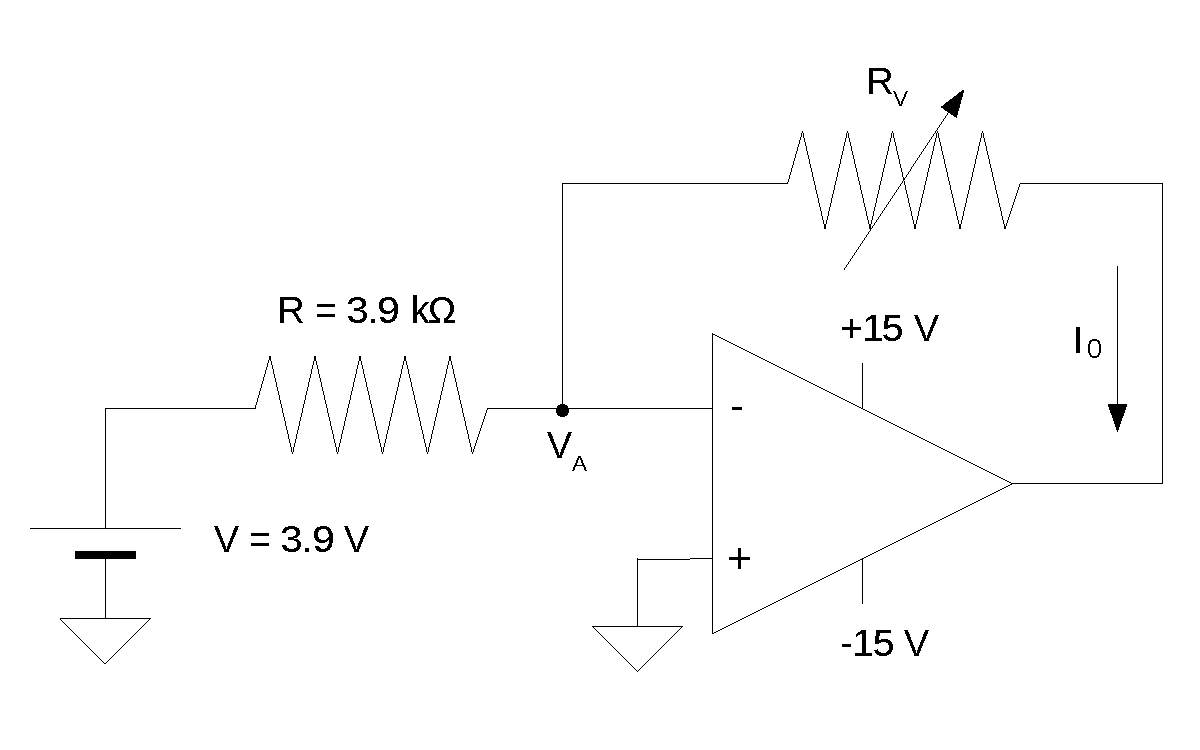
\includegraphics[width=\textwidth]{../figure/schema_gen_corr.pdf}
                \caption{Generatore di corrente costante}
                \label{fig:generatore}
        \end{subfigure}
        ~
        \begin{subfigure}[b]{0.48\textwidth}
                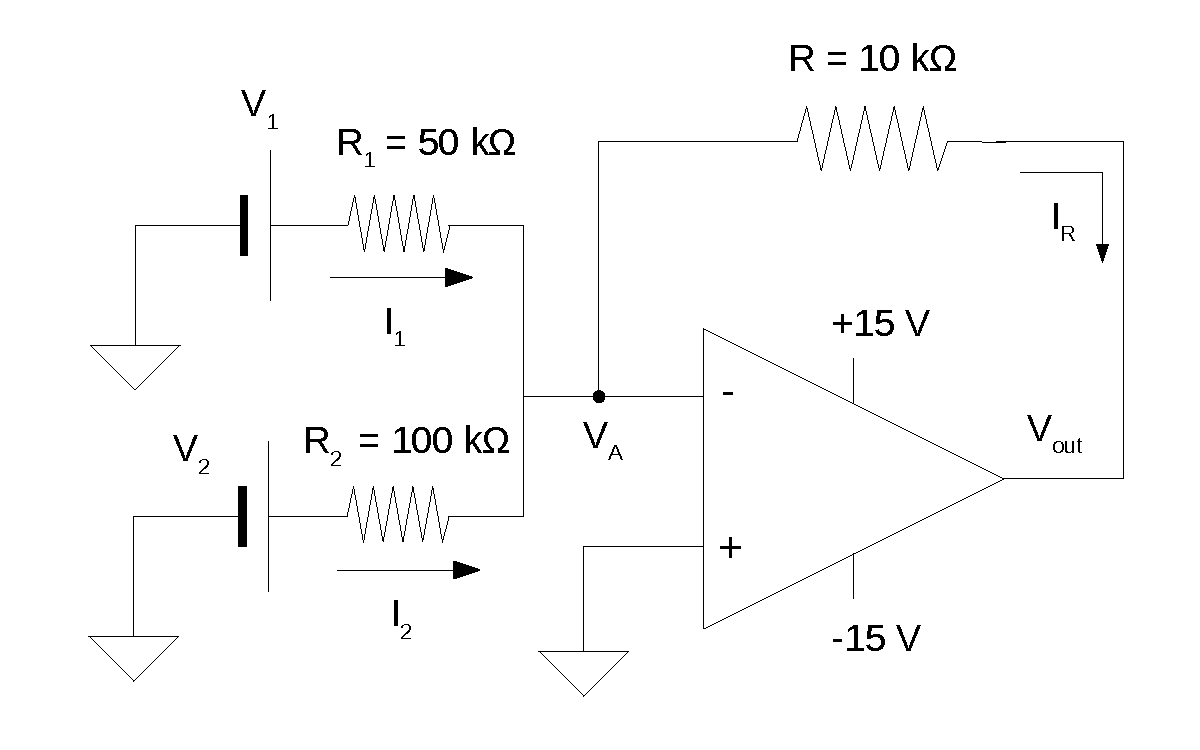
\includegraphics[width=\textwidth]{../figure/circuito_sommatore.pdf}
                \caption{Sommatore pesato di tensioni}
                \label{fig:sommatore}
        \end{subfigure}
        \caption{Circuiti costruiti durante l'esperienza. Il primo è un generatore di corrente costante, mentre il secondo è un sommatore pesato di segnali in ingresso.}
        \label{fig:circuits}
\end{figure}